\clearpage \section{Horizontal Stretching}
Horizontal stretching is by far the most confusing. At the beginning of this chapter, I wrote $\dfrac{1}{b}(x - h)$ and noted that some texts use $b$ instead of $\dfrac{1}{b}$. In this section, I'll be sure to clarify exactly what adding a value in front of those parentheses does to the function and explain the differences between $b$ and $\dfrac{1}{b}$. 

Let's define a function $f(x) = x^2$. I'll now create a table with three columns: one for the $x$ value plugged into the function, one for the value of $x$ after $b$ is applied, and one for the output of the function. In this case, $b = 1$, so the table of $f(x)$ looks something like this:
\begin{center}
    \begin{tabular}{ c | c | c }
        $x$ & $1x$ & $f(x)$ \\
        \hline
        $-2$ & $-2$ & $4$ \\
        \hline
        $-1$ & $-1$ & $1$ \\
        \hline
        $0$ & $0$ & $0$ \\
        \hline
        $1$ & $1$ & $1$ \\
        \hline
        $2$ & $2$ & $4$
    \end{tabular}\\
\end{center}
Now let's look at another function $g(x) = (2x)^2$.
\begin{center}
    \begin{tabular}{ c | c | c }
        $x$ & $2x$ & $g(x)$ \\
        \hline
        $-2$ & $-4$ & $16$ \\
        \hline
        $-1$ & $-2$ & $4$ \\
        \hline
        $0$ & $0$ & $0$ \\
        \hline
        $1$ & $2$ & $4$ \\
        \hline
        $2$ & $4$ & $16$
    \end{tabular}\\
\end{center}
Notice how an input of $2$ all of a sudden becomes $4$. This is \textit{almost} like a vertical stretch. If this \textit{had} been a vertical stretch (i.e. $y = 2x^2$), an input of $2$ would produce $y = 8$. But we got $16$ this time with $g(x)$. Instead of imagining it as a stretch upward, imagine the graph being smushed together so that the points are more tightly packed near the $y$-axis line ($x = 0$).

Btw, you could totally see it as something similar to a vertical stretch. Your teacher might not like it (and neither do I) because doing so would make it easy to confuse the vertical stretch $2x^2$ with the "vertical stretch" $(2x)^2$. So, just for teacher's and your own sanity, just think of $(2x)^2$ as a horizontal compression.

Let's look at these functions on a graph!
\begin{center}
    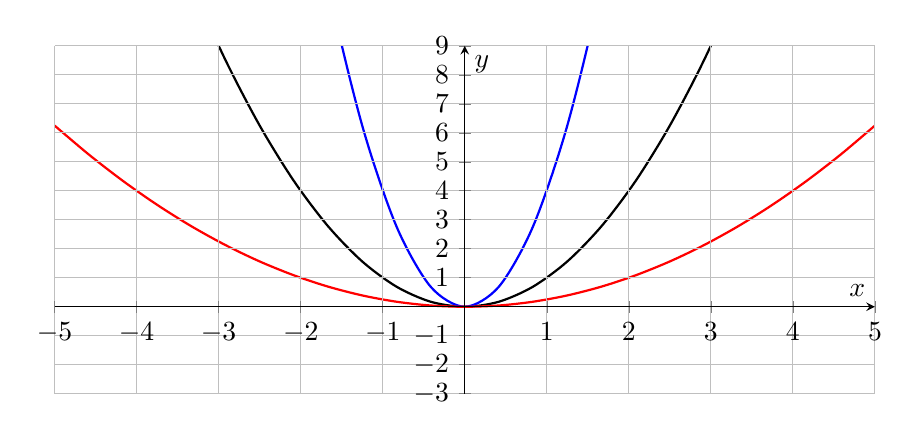
\begin{tikzpicture}
        \begin{axis} [
            axis lines=middle,
            xlabel = $x$, ylabel = {$y$},
            xmin = -5, xmax = 5,
            ymin = -3, ymax = 9,
            xtick distance={1}, ytick distance={1},
            grid = both,
            width = 12cm,
            height = 6cm,
            smooth,
            axis on top
        ]
        \addplot[black, thick, domain=-5:5] {x^2};
        \addplot[blue, thick, domain=-5:5] {(2 * x)^2};
        \addplot[red, thick, domain=-5:5] {((1/2) * x)^2};
        \end{axis}
    \end{tikzpicture}\\
    $f(x) = x^2$ (Black), $g(x) = (2x)^2$ (Blue), $\displaystyle h(x) = \left(\dfrac{1}{2}x\right)^2$ (Red)
\end{center}

\begin{definition}
    Given a function $f(x)$ and a horizontal stretch $b$, the new function $\displaystyle g(x) = f\left(\dfrac{1}{b}x\right)$ is the function of $f$ horizontally stretched by a factor of $b$.
    \begin{itemize}
        \item When $b > 1$, horizontal stretching occurs.
        \item When $0 < b < 1$, horizontal compression occurs.
        \item When $b = 1$, the function is unaffected.
        \item When $b = 0$, the function is undefined.
    \end{itemize}
\end{definition}